\documentclass[10pt,a4paper,twocolumn]{article}

\usepackage[utf8]{inputenc}
\usepackage[T1]{fontenc}
\usepackage[hmargin=1.6cm,top=1.4cm,bottom=1.6cm]{geometry}
\linespread{0.96}
\usepackage{times}
\usepackage{titlesec}
\usepackage{microtype}
\usepackage{url}
\urlstyle{same}
\usepackage{graphicx}
\usepackage{xcolor}
\usepackage{booktabs}
\usepackage{capt-of}
\usepackage{tikz}
\usetikzlibrary{arrows.meta,positioning}
\definecolor{atanavy}{HTML}{2A2660}
\usepackage[superscript]{cite}
\makeatletter
\renewcommand{\@citess}[1]{\textsuperscript{[#1]}}
\makeatother
\usepackage[hidelinks]{hyperref}
\usepackage[font=small,labelfont=bf,skip=4pt]{caption}

\titleformat{\section}{\normalsize\bfseries\color{atanavy}}{\thesection.}{0.5em}{}
\titlespacing*{\section}{0pt}{1.0ex plus 0.3ex}{0.5ex}
\setlength{\parskip}{0.3ex}

\title{\vspace{-1.6cm}
\includegraphics[height=1.3cm]{atauni-logo.png}\\[0.6em]\Large\textbf{Emotion-Driven VTuber Avatars: Comparing Deep Learning Models for Facial Emotion Recognition}}
\author{Ömer Sunguralp Bektaş \\
\small Artificial Intelligence and Data Engineering, Atatürk University, Erzurum, Türkiye \\
\small \href{mailto:omersunguralp.bektas24@ogr.atauni.edu.tr}{omersunguralp.bektas24@ogr.atauni.edu.tr} \enspace$\cdot$\enspace ORCID: \href{https://orcid.org/0009-0000-8254-4949}{0009-0000-8254-4949}}
\date{}

\begin{document}
\maketitle

\section{Problem Statement}
In this project, I aim to build a system that recognises emotions from the face in order to change the expression of a VTuber model automatically. The input of the system is video, so that it can also be used during live streams. At the output, the system assigns the live image to one of several emotion categories, and the predicted category changes the expression of the avatar model (Figure~\ref{fig:system}). The planned categories are seven emotions: neutral, happy, sad, angry, fearful, disgusted and surprised. The problem is therefore a multi-class classification problem.

Understanding emotion from the face with hand-written rules is difficult, because every person's face and way of showing emotion is different. A familiar example is the Turkish football manager Fatih Terim, who conveys with his lips and the area around them the emotions that most people express with their eyebrows and the area around them. Moreover, every person interprets an expression differently. A deep learning method can learn this without the need for such hand-written rules.

Two different approaches will be compared. The first is a frame-based model that extracts the frames of the videos in the dataset one by one and predicts the emotion from these images. The second is a model that processes the data as a sequence, so that consecutive frames can be evaluated together without breaking their temporal order. The main aim is to see the effect of temporal change on the model and to understand which of the two is usable in a live-streaming system.

\section{Motivation}
A VTuber, in full ``Virtual YouTuber'', is a content creator who produces content on the internet with a virtual character instead of showing their face. Pre-designed 2D or 3D models are made to move by means of various body-tracking systems. Today, many content creators, both newcomers and those with a considerable audience, use models of this kind. Existing VTuber software such as VTube Studio~\cite{vtubestudio} already tracks the face with a webcam and transfers its movements to the model, but the special expressions of the model are still switched on and off manually, with hotkeys or with additional devices such as a Stream Deck, both in live streams and in video recordings. With an emotion recognition system, this project aims to make this process automatic.

Deep learning is now widely used for facial expression recognition~\cite{lideng}. On the dataset used in this project, Luna-Jim\'enez et al.~\cite{luna} reported that frame-based systems can have problems when they are applied directly to a video-based task. Building on this observation, this project compares the two approaches in a controlled way, using only the visual modality, and also considers running speed for a live application.

\vspace{1.2ex}
\begin{center}
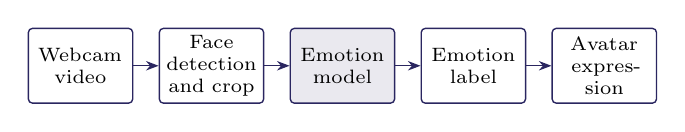
\begin{tikzpicture}[
  node distance=3.2mm,
  box/.style={draw=atanavy, rounded corners=1.5pt, line width=0.5pt,
              minimum height=9.5mm, text width=12.2mm, align=center,
              font=\scriptsize, inner sep=1.5pt},
  arr/.style={-{Stealth[length=1.6mm]}, draw=atanavy, line width=0.5pt}]
  \node[box] (cam) {Webcam video};
  \node[box, right=of cam] (face) {Face detection and crop};
  \node[box, right=of face, fill=atanavy!10] (model) {Emotion model};
  \node[box, right=of model] (label) {Emotion label};
  \node[box, right=of label] (avatar) {Avatar expression};
  \draw[arr] (cam) -- (face);
  \draw[arr] (face) -- (model);
  \draw[arr] (model) -- (label);
  \draw[arr] (label) -- (avatar);
\end{tikzpicture}
\captionof{figure}{Overview of the planned system.}\label{fig:system}
\end{center}

\newpage % sutun sonu: bolum bolunmesin
\section{Dataset}
\enlargethispage{1.2\baselineskip}
For this project I chose the RAVDESS dataset (Ryerson Audio-Visual Database of Emotional Speech and Song)~\cite{ravdess}. The first reason for choosing this dataset was that it is openly available and free to use. The dataset can be accessed on Zenodo and has a CC BY-NC-SA 4.0 licence, which means there is no problem as long as I do not use it commercially.

The dataset contains 24 different professional actors in total, 12 male and 12 female. For each of them there are videos in which they say two fixed sentences with different emotions. Every video has a resolution of $1280\times720$ at 30 frames per second. In this project I will use only the visual part of the videos; the audio will not be included. This part contains 1,440 clips, 60 per actor. The dataset itself has eight emotions, but because neutral and calm are very similar to each other, I will merge them and reduce the number of emotions to seven. The neutral class will then have 288 clips and each of the other emotions 192 clips.

The second reason for choosing this dataset is that, because it contains video, I will be able to compare the two approaches I have in mind on a single dataset.

I will split the dataset actor by actor: 16 actors will be used for training, 4 for validation and 4 for testing. The clips of one actor will be used for only one purpose, so that during testing the model also meets faces it has not seen.

\section{Proposed Methodology}
First, I need to prepare the dataset. From every clip I will extract a fixed number of frames at equal intervals, extract the face region from the frames with an existing face detection tool, and resize the extracted faces to the size expected by the model.

After that, I will build the models from simple to complex. I first need to train a simple CNN. I will then build my frame-based models with two different pretrained CNNs, and after that four sequence-based models, which use temporal information on top of these CNNs.

In the experiments I will consider three factors: the number of frames the model looks at together, the difference between starting from pretrained weights and training from scratch, and the effect of using data augmentation. To understand the effect of these factors more clearly, I will change only one factor in each experiment. These experiments will be carried out on a single main model.

When examining the results of these experiments, I will interpret the reasons for the errors through examples that the model predicts correctly and incorrectly. With the Grad-CAM method~\cite{gradcam}, I will also understand which region of the face the model looks at when making a decision. In addition, I will visualise the attention weights of the Transformer models to show which frames of a clip they focus on. Finally, I will connect the most suitable model to a camera system and prepare a demo that changes the VTuber model according to the predicted emotion.

\newpage % sutun sonu: bolum bolunmesin
\section{Baseline}
The basic model I will use to compare the models will be a simple CNN with a few layers, trained from scratch. This model will check the frames obtained from the videos one by one and predict a suitable emotion for each of them. To find the emotion of a clip, it will check all the frames extracted from that clip and take the most frequently repeated emotion as its prediction. Because this model is not pretrained and does not use temporal information, I will examine how much it differs from the other models.

\section{Planned Deep Learning Models}
Following the logic of the two approaches described earlier, I will build six models besides the baseline (Table~\ref{tab:models}).

In the frame-based approach I will use two CNNs pretrained on ImageNet: ResNet-18~\cite{resnet} and MobileNetV2~\cite{mobilenetv2}. For both, I will replace the output layer according to the seven emotion classes and train them on my own data. Like the baseline, these models will make a separate prediction for every frame and take the most frequently repeated emotion as the prediction for the clip. The reason for choosing two different CNNs is that ResNet-18 is more powerful but heavier, while MobileNetV2 is lighter and faster. In this way I will see the trade-off between speed and accuracy.

In the sequence-based approach I will use both CNNs to extract features from every frame and pass these features, without breaking the order of the frames, to a layer that processes temporal information. For this layer I will follow two different ideas with each CNN: an LSTM~\cite{lstm}, which reads the frames in order, and a Transformer~\cite{transformer}, which looks at all frames at the same time. Because my dataset is relatively small, I will keep the Transformers to a small number of layers to reduce the risk of overfitting. These four models will produce a single emotion prediction for every clip.

\section{Evaluation Metrics}
To evaluate the models I will use accuracy, precision, recall and F1-score, and I will produce a confusion matrix for every model. Because the number of clips is not equal across the classes, I will take the macro F1-score, which gives equal weight to every class, as the main evaluation measure. All models will be evaluated on the same test actors and at clip level, so that the results are directly comparable. Because the dataset is small and the test set contains only four actors, the fixed split will be used for the experiments, and the final comparison of the models will additionally be repeated with actor-wise cross-validation, reporting the mean and standard deviation of the results. Using the confusion matrix, I will examine which emotions are confused with each other. To measure usability in a live stream, I will also report how many frames per second each model can process. During training I will follow the training and validation loss curves to check whether the model is overfitting.

\section{Expected Contribution}
At the end of this project I expect to present three things. The first is a comparison of the frame-based and sequence-based approaches on the same dataset and the same test actors; through this I will show how much temporal information contributes to emotion recognition. The second is an examination of the trade-off between the accuracy of the models and their running speed, which will allow me to say which model is suitable for live streaming. The third is a working demo that automatically changes the expression of a VTuber model using only a camera. In addition, through error analysis and explainability methods, I will show in which emotions the models struggle and why.

\newpage % sutun sonu: bolum bolunmesin
\begin{center}
\captionof{table}{Models to be compared.}\label{tab:models}
\small\setlength{\tabcolsep}{2.5pt}
\begin{tabular}{@{}llcc@{}}
\toprule
Approach & Model & Pretrained & Temporal \\
\midrule
Baseline       & Simple CNN              & No  & No  \\
Frame-based    & ResNet-18               & Yes & No  \\
Frame-based    & MobileNetV2             & Yes & No  \\
Sequence-based & ResNet-18 + LSTM        & Yes & Yes \\
Sequence-based & ResNet-18 + Transformer & Yes & Yes \\
Sequence-based & MobileNetV2 + LSTM        & Yes & Yes \\
Sequence-based & MobileNetV2 + Transformer & Yes & Yes \\
\bottomrule
\end{tabular}
\end{center}
\vspace{1ex}

{\small
\begin{thebibliography}{9}
\setlength{\itemsep}{0pt}

\bibitem{vtubestudio}
DenchiSoft, ``VTube Studio documentation,'' \url{https://github.com/DenchiSoft/VTubeStudio/wiki}, accessed Oct.~2026.

\bibitem{lideng}
S.~Li and W.~Deng, ``Deep facial expression recognition: A survey,'' \emph{IEEE Trans. Affective Computing}, vol.~13, no.~3, pp.~1195--1215, 2022.

\bibitem{luna}
C.~Luna-Jim\'enez, D.~Griol, Z.~Callejas, R.~Kleinlein, J.~M. Montero, and F.~Fern\'andez-Mart\'inez, ``Multimodal emotion recognition on RAVDESS dataset using transfer learning,'' \emph{Sensors}, vol.~21, no.~22, 7665, 2021.

\bibitem{ravdess}
S.~R. Livingstone and F.~A. Russo, ``The Ryerson Audio-Visual Database of Emotional Speech and Song (RAVDESS): A dynamic, multimodal set of facial and vocal expressions in North American English,'' \emph{PLoS ONE}, vol.~13, no.~5, e0196391, 2018.

\bibitem{gradcam}
R.~R. Selvaraju, M.~Cogswell, A.~Das, R.~Vedantam, D.~Parikh, and D.~Batra, ``Grad-CAM: Visual explanations from deep networks via gradient-based localization,'' in \emph{Proc. IEEE ICCV}, 2017, pp.~618--626.

\bibitem{resnet}
K.~He, X.~Zhang, S.~Ren, and J.~Sun, ``Deep residual learning for image recognition,'' in \emph{Proc. IEEE CVPR}, 2016, pp.~770--778.

\bibitem{mobilenetv2}
M.~Sandler, A.~Howard, M.~Zhu, A.~Zhmoginov, and L.-C. Chen, ``MobileNetV2: Inverted residuals and linear bottlenecks,'' in \emph{Proc. IEEE CVPR}, 2018, pp.~4510--4520.

\bibitem{lstm}
S.~Hochreiter and J.~Schmidhuber, ``Long short-term memory,'' \emph{Neural Computation}, vol.~9, no.~8, pp.~1735--1780, 1997.

\bibitem{transformer}
A.~Vaswani et al., ``Attention is all you need,'' in \emph{Advances in Neural Information Processing Systems}, vol.~30, 2017.

\end{thebibliography}
}

\end{document}
